% Provenance (never printed): cycle 4 SVT/physique, "La planete Terre,
% l'environnement": the movements of the atmosphere, weather and its
% forecast; see sources/book1/PROVENANCE.md. Book 1, grade 8, chapter 3.
% Vocabulary guard: owns air mass, front (warm, cold), depression (homograph:
% phrase-level linking only), anticyclone, isobar, weather forecast. The
% rotation of the winds around lows and highs is told (deflection, recalled
% from ch. g8.2); the occluded front is named in prose only; numerical models
% are told, not taught.
\chapter{Luchtmassa's, fronten en weerkaarten}\label{ch:g8:fronts-and-weather-maps}

De ochtend is helder en windstil. Rond het middaguur verschijnen er heel
hoog in de lucht dunne witte strepen, die zich langzaam uitspreiden tot een
bleke sluier die de Zon dof maakt. In de middag worden de \omterm{def:g4:clouds-rain-snow:cloud}{wolken} dikker en
komen ze lager; tegen de avond valt er een gestage \omterm{def:g4:clouds-rain-snow:precipitation}{regen}. In de nacht wordt
het warm en vochtig, en dan brengt een donkere wolkenband een korte, hevige
bui en een windstoot. De volgende ochtend is helder, fris en winderig. In
twee dagen is er een \emph{\omterm{def:g8:fronts-and-weather-maps:depression}{depressie}} met haar twee \omterm{def:g8:fronts-and-weather-maps:front}{fronten} over de stad
getrokken.
% ledger: ucar:warm-front, ucar:cold-front

\begin{omfigure}
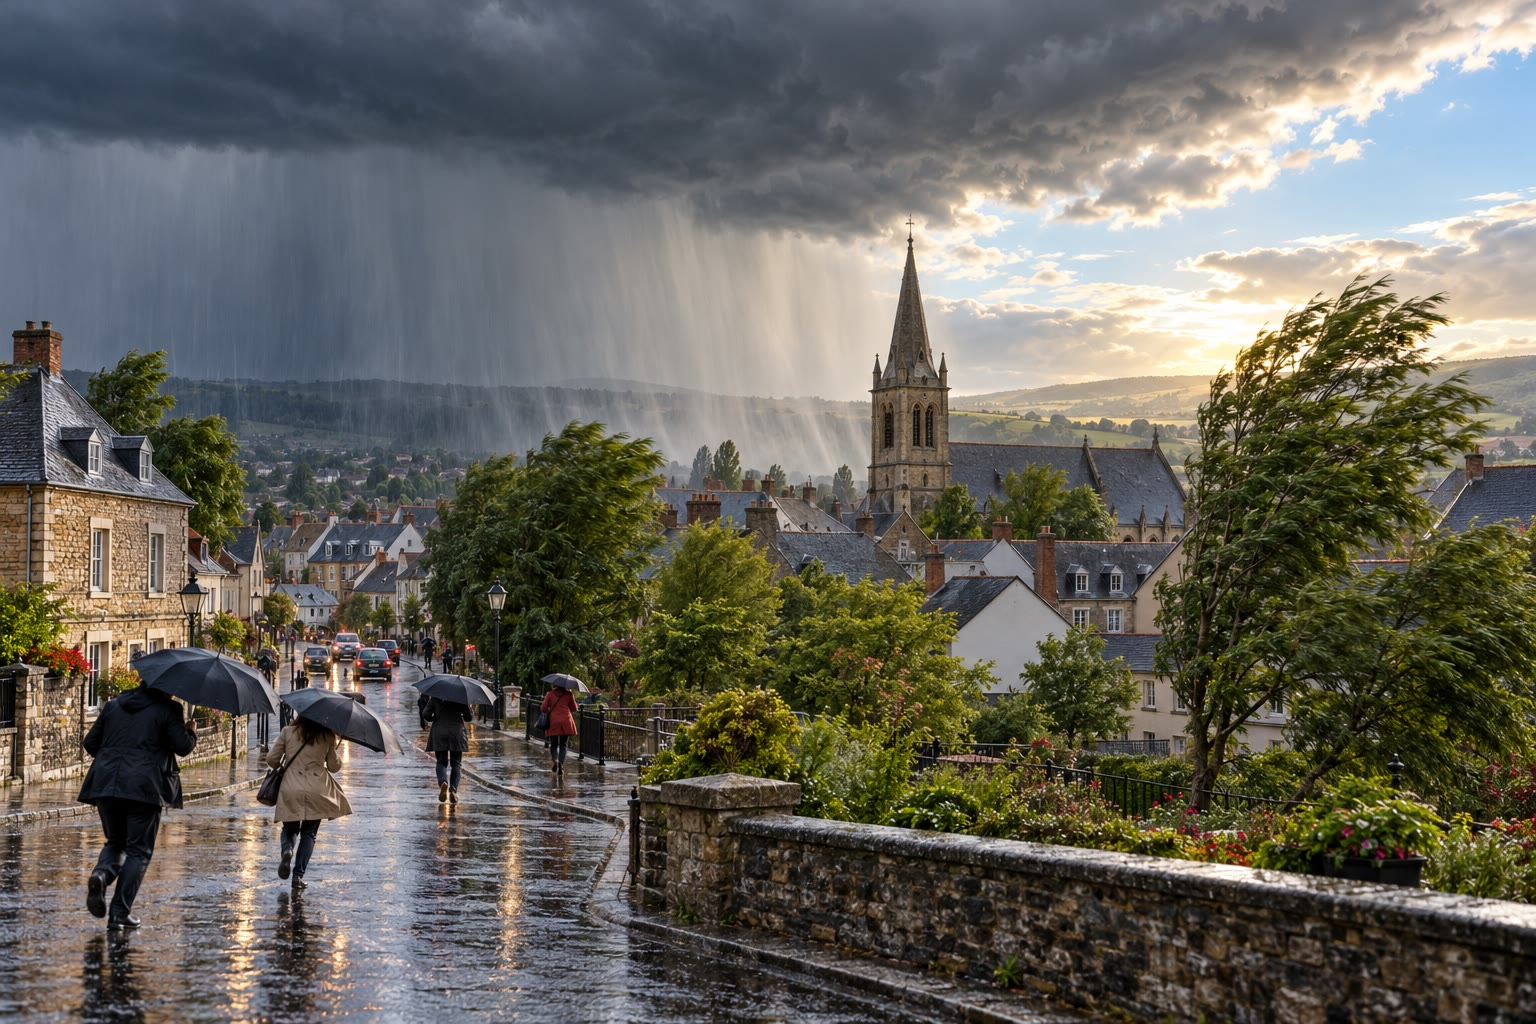
\includegraphics[width=0.6\linewidth]{images/book1/ai/g8-rain-arriving.jpg}

{\small Een regengordijn trekt onder een donkere wolkenbasis over een
stad, terwijl de lucht achter de kerk nog helder is (door AI gegenereerde
illustratie van een algemene scène).}
\label{fig:g8:fronts-and-weather-maps:rain}
\end{omfigure}

Weervoorspellers zagen het dagen van tevoren aankomen. Dit hoofdstuk laat
zien hoe: de lucht boven ons komt in grote massa's, de massa's ontmoeten
elkaar langs \omterm{def:g8:fronts-and-weather-maps:front}{fronten}, en \omterm{def:g2:drawing-to-map:map}{kaarten} van de luchtdruk tonen waar ze naartoe
gaan.

\begin{recall}
Lucht drukt op alles wat ze raakt; een barometer meet deze druk in
hectopascal (de natuurkundeboeken), en op \omterm{def:g4:world-physical-map:altitude}{zeeniveau} is hij ongeveer
\qty{1013}{hPa} (\cref{ch:g8:the-atmosphere}). \omterm{def:g4:clouds-rain-snow:cloud}{Wolken} ontstaan als vochtige
lucht opstijgt en afkoelt (\cref{ch:g4:clouds-rain-snow}). Aan de grond
waait de wind van hoge druk naar lage druk, en de draaiing van de Aarde
buigt hem af: naar rechts op het \omterm{def:g3:continents-and-oceans:equator}{noordelijk halfrond}. Tussen ongeveer
\ang{30} en \ang{60} brengen de \omterm{def:g8:winds-global-circulation:global-winds}{westenwinden} de ene \omterm{def:g5:natural-hazards:storm}{storm} na de andere
(\cref{ch:g8:winds-global-circulation}).
\end{recall}

\section{Luchtmassa's}

Lucht die dagenlang boven dezelfde plek blijft, neemt het karakter aan van
het oppervlak eronder. Boven een warme \omterm{def:g2:water-on-earth:ocean}{oceaan} wordt ze warm en vochtig;
boven bevroren land koud en droog. Als ze wegtrekt, neemt ze dit karakter
mee, soms over duizenden kilometers.
% ledger: noaa:air-mass

\begin{definition}[Luchtmassa]\label{def:g8:fronts-and-weather-maps:air-mass}
Een \emph{luchtmassa}\index{luchtmassa} is een heel grote hoeveelheid lucht
waarin de temperatuur en de vochtigheid op een gegeven hoogte overal
ongeveer gelijk zijn. Ze krijgt die van het gebied waar ze ontstond, haar
\emph{brongebied}.
\end{definition}
% ledger: noaa:air-mass

Weervoorspellers geven een \omterm{def:g8:fronts-and-weather-maps:air-mass}{luchtmassa} een naam van twee letters. De eerste
zegt waar ze ontstond: \emph{c} (continentaal) boven land, dus is ze droog;
\emph{m} (maritiem) boven een \omterm{def:g2:water-on-earth:ocean}{oceaan}, dus is ze vochtig. De tweede zegt hoe
koud ze is: \emph{A} (arctisch) boven de poolgebieden, \emph{P} (polair)
boven de hoge breedten, \emph{T} (tropisch) boven de lage breedten. Lucht
uit een hete \omterm{def:g5:weather-and-climate:desert}{woestijn} is cT, heet en droog; lucht uit het Noordpoolgebied
is cA, heel koud en droog.
% ledger: noaa:air-mass

\begin{omfigure}
\begin{tikzpicture}
\begin{axis}[ommap, width=12.6cm, xmin=-100, xmax=60, ymin=10, ymax=85,
  xtick={-90,-60,...,60}, ytick={20,40,60,80},
  xticklabels={$90^\circ$WL,$60^\circ$WL,$30^\circ$WL,$0^\circ$,$30^\circ$OL,$60^\circ$OL},
  yticklabels={$20^\circ$NB,$40^\circ$NB,$60^\circ$NB,$80^\circ$NB},
  tick label style={font=\scriptsize}]
  \addplot[fill=omLithAlluv, draw=black!45, line width=0.2pt] table {figdata/out/shared-geo-land.dat};
  \tikzset{src/.style={line width=0.9pt, fill opacity=0.35, text opacity=1, font=\scriptsize, align=center}}
  \draw[src, draw=omCold, fill=omCold!35] (axis cs:-30,79) ellipse [x radius=26, y radius=4.5];
  \node[font=\scriptsize, align=center, fill=white, inner sep=1pt] at (axis cs:-30,79) {\textbf{cA}: heel koud, droog};
  \draw[src, draw=omCold, fill=omCold!25] (axis cs:-35,55) ellipse [x radius=14, y radius=6];
  \node[font=\scriptsize, align=center, fill=white, inner sep=1pt] at (axis cs:-35,55) {\textbf{mP}: koud,\\ vochtig};
  \draw[src, draw=omCold, fill=omCold!25] (axis cs:-84,60) ellipse [x radius=12, y radius=7];
  \node[font=\scriptsize, align=center, fill=white, inner sep=1pt] at (axis cs:-84,60) {\textbf{cP}: koud,\\ droog};
  \draw[src, draw=omCold, fill=omCold!25] (axis cs:45,62) ellipse [x radius=14, y radius=7];
  \node[font=\scriptsize, align=center, fill=white, inner sep=1pt] at (axis cs:45,62) {\textbf{cP}: koud,\\ droog};
  \draw[src, draw=omWarm, fill=omWarm!25] (axis cs:-45,28) ellipse [x radius=16, y radius=6];
  \node[font=\scriptsize, align=center, fill=white, inner sep=1pt] at (axis cs:-45,28) {\textbf{mT}: warm,\\ vochtig};
  \draw[src, draw=omWarm, fill=omWarm!25] (axis cs:10,24) ellipse [x radius=15, y radius=6];
  \node[font=\scriptsize, align=center, fill=white, inner sep=1pt] at (axis cs:10,24) {\textbf{cT}: heet,\\ droog};
\end{axis}
\end{tikzpicture}

{\small Typische brongebieden van \omterm{def:g8:fronts-and-weather-maps:air-mass}{luchtmassa's} rond de noordelijke
Atlantische \omterm{def:g2:water-on-earth:ocean}{Oceaan} (schematisch): boven het Noordpoolgebied, de koude
\omterm{def:g3:continents-and-oceans:continent}{continenten}, de noordelijke \omterm{def:g2:water-on-earth:ocean}{oceaan}, de subtropische \omterm{def:g2:water-on-earth:ocean}{oceaan} en de Sahara.
Blauw: koude \omterm{def:g8:fronts-and-weather-maps:air-mass}{luchtmassa's}; rood: warme.}
% ledger: noaa:air-mass, data:ne-land (schematic regions)
\label{fig:g8:fronts-and-weather-maps:sources}
\end{omfigure}

\section{Fronten}

Als een \omterm{def:g8:fronts-and-weather-maps:air-mass}{luchtmassa} zich verplaatst, ontmoet ze een andere. De twee mengen
niet gemakkelijk: ze blijven gescheiden, met een smalle grens ertussen waar
het \omterm{def:g1:watching-the-weather:weather}{weer} verandert.
% ledger: mo:fronts, ucar:cold-front

\begin{definition}[Front]\label{def:g8:fronts-and-weather-maps:front}
Een \emph{front}\index{front} is de grens aan de grond tussen twee
\omterm{def:g8:fronts-and-weather-maps:air-mass}{luchtmassa's} met een verschillende temperatuur en vochtigheid. Bij een
\emph{koufront}\index{koufront} dringt koude lucht in warmere lucht en
neemt ze haar plaats in; bij een \emph{warmtefront}\index{warmtefront}
dringt warme lucht in koudere lucht en neemt ze haar plaats in.
\end{definition}
% ledger: mo:fronts, ucar:cold-front, ucar:warm-front

Koude lucht is dichter dan warme lucht. Bij een \omterm{def:g8:fronts-and-weather-maps:front}{koufront} schuift de koude
lucht als een wig onder de warme lucht en tilt die steil omhoog. De warme,
vochtige lucht stijgt snel op en bouwt hoog oprijzende \omterm{def:g4:clouds-rain-snow:cloud}{wolken}, \omterm{def:g4:clouds-rain-snow:cloud-families}{cumulus} en
\omterm{def:g4:clouds-rain-snow:cloud-families}{cumulonimbus}: het \omterm{def:g8:fronts-and-weather-maps:front}{front} brengt hevige buien, soms \omterm{def:g4:clouds-rain-snow:precipitation}{hagel} en onweer,
windstoten en een plotselinge daling van de temperatuur. Als het voorbij
is, houdt de \omterm{def:g4:clouds-rain-snow:precipitation}{regen} op en klaart de lucht op. Een \omterm{def:g8:fronts-and-weather-maps:front}{koufront} verplaatst zich
snel, tot twee keer zo snel als een \omterm{def:g8:fronts-and-weather-maps:front}{warmtefront}.
% ledger: ucar:cold-front

\begin{omfigure}
\begin{tikzpicture}[font=\footnotesize, >={Stealth[length=2.2mm]}, yscale=0.7, xscale=0.95]
  % ground
  \draw[line width=0.8pt] (0,0) -- (15,0);
  % cold wedge, nose at x = 8.2
  \fill[omCold!18] (0,0) -- (0,3.4) .. controls (4.5,3.2) and (7.2,2.4) .. (7.9,0.8)
    .. controls (8.1,0.35) and (8.2,0.12) .. (8.25,0) -- cycle;
  \draw[omCold, line width=1pt] (0,3.4) .. controls (4.5,3.2) and (7.2,2.4) .. (7.9,0.8)
    .. controls (8.1,0.35) and (8.2,0.12) .. (8.25,0);
  \node[omCold, align=center] at (3.2,1.4) {\textbf{koude lucht}\\(dicht)};
  \node[omWarm, align=center] at (12.6,1.4) {\textbf{warme,}\\\textbf{vochtige lucht}};
  % cold air pushes
  \draw[->, omCold, line width=1.2pt] (4.6,0.5) -- (7.0,0.5);
  % warm air lifted
  \draw[->, omWarm, line width=1.2pt] (11.2,0.45) .. controls (9.4,0.6) and (8.6,1.4) .. (8.5,3.0);
  % cumulonimbus
  \fill[black!12] (7.3,2.6) .. controls (7.0,3.4) and (7.4,4.2) .. (7.9,4.5)
    .. controls (7.6,5.0) and (8.6,5.2) .. (9.4,5.1) -- (11.0,5.15)
    .. controls (10.6,4.9) and (10.2,4.8) .. (10.0,4.6)
    .. controls (10.4,4.0) and (10.2,3.0) .. (9.8,2.5) -- cycle;
  \draw[black!45] (7.3,2.6) .. controls (7.0,3.4) and (7.4,4.2) .. (7.9,4.5)
    .. controls (7.6,5.0) and (8.6,5.2) .. (9.4,5.1) -- (11.0,5.15)
    .. controls (10.6,4.9) and (10.2,4.8) .. (10.0,4.6)
    .. controls (10.4,4.0) and (10.2,3.0) .. (9.8,2.5) -- cycle;
  \node at (9.0,3.8) {cumulonimbus};
  \foreach \x in {7.7,8.0,...,9.6} \draw[omCold!70, line width=0.5pt] (\x,2.45) -- (\x-0.25,0.15);
  \node[anchor=west, align=left] at (9.8,1.95) {hevige buien,\\windstoten};
  % motion
  \draw[->, line width=1.3pt] (5.7,4.3) -- (7.2,4.3);
  \node[anchor=east] at (5.6,4.3) {het front verplaatst zich};
  \node[anchor=north] at (8.25,-0.1) {front aan de grond};
  \node[anchor=north west, align=left] at (0.1,-0.1) {erachter: koeler, opklarend};
  \node[anchor=north east, align=right] at (15,-0.1) {ervoor: warm, vochtig};
\end{tikzpicture}

{\small Een \omterm{def:g8:fronts-and-weather-maps:front}{koufront} van opzij gezien (hoogten sterk overdreven). De koude
lucht schuift als een wig onder de warme lucht; de warme lucht wordt steil
opgetild en bouwt hoog oprijzende \omterm{def:g4:clouds-rain-snow:cloud}{wolken}.}
% ledger: ucar:cold-front
\label{fig:g8:fronts-and-weather-maps:cold}
\end{omfigure}

Bij een \omterm{def:g8:fronts-and-weather-maps:front}{warmtefront} kan de lichte warme lucht de koude lucht niet van de
grond wegduwen: ze klimt er langzaam overheen, langs een lange en flauwe
helling. Haar \omterm{def:g4:clouds-rain-snow:cloud}{wolken} verschijnen daarom ver voor het \omterm{def:g8:fronts-and-weather-maps:front}{front} uit, hoog in de
lucht: eerst dunne strepen \omterm{def:g4:clouds-rain-snow:cloud-families}{cirrus}, dan een sluier van cirrostratus, dan
grijze altostratus. Naarmate het \omterm{def:g8:fronts-and-weather-maps:front}{front} dichterbij komt, worden de \omterm{def:g4:clouds-rain-snow:cloud}{wolken}
lager en dikker en begint een lange, gestage \omterm{def:g4:clouds-rain-snow:precipitation}{regen}. Als het voorbij is,
is de lucht warmer en vochtiger.
% ledger: ucar:warm-front, bom:isobars (warm front: steady rain, grey skies)

\begin{omfigure}
\begin{tikzpicture}[font=\footnotesize, >={Stealth[length=2.2mm]}]
  \draw[line width=0.8pt] (0,0) -- (15,0);
  % cold air ahead (right), warm air climbing a gentle slope from the front at x = 2.2
  \fill[omCold!18] (2.2,0) .. controls (6,0.9) and (10,2.2) .. (15,3.4) -- (15,0) -- cycle;
  \draw[omCold, line width=1pt] (2.2,0) .. controls (6,0.9) and (10,2.2) .. (15,3.4);
  \node[omCold, align=center] at (11.8,0.75) {\textbf{koude lucht}};
  \node[omWarm, align=center] at (1.4,1.6) {\textbf{warme,}\\\textbf{vochtige lucht}};
  \draw[->, omWarm, line width=1.2pt] (1.0,0.45) .. controls (4.5,0.9) and (8.5,2.4) .. (12.4,3.4);
  % clouds: nimbostratus near the front, altostratus, cirrostratus, cirrus far ahead
  \fill[black!18] (2.4,0.7) .. controls (3.2,1.8) and (5.5,2.3) .. (6.6,2.4) -- (6.4,1.25) .. controls (5,1.0) and (3.8,0.7) .. cycle;
  \node at (5.4,1.62) {nimbostratus};
  \foreach \x in {3.0,3.3,...,5.7} \draw[omCold!70, line width=0.5pt] (\x,0.95) -- (\x-0.2,0.25);
  \fill[black!10, rounded corners=4pt] (6.4,2.65) rectangle (10.0,3.25);
  \node at (8.2,2.95) {altostratus};
  \fill[black!6, rounded corners=4pt] (9.6,3.75) rectangle (12.6,4.15);
  \node at (11.1,3.95) {cirrostratus};
  \foreach \x in {12.6,13.2,13.8} \draw[black!35, line width=0.6pt] (\x,4.55) .. controls (\x+0.2,4.75) and (\x+0.4,4.6) .. (\x+0.55,4.85);
  \node[anchor=south] at (13.4,4.9) {cirrus};
  \draw[->, line width=1.3pt] (2.6,4.3) -- (4.1,4.3);
  \node[anchor=east] at (2.5,4.3) {het front verplaatst zich};
  \node[anchor=north] at (2.2,-0.1) {front aan de grond};
  \node[anchor=north east] at (15,-0.1) {ver vooruit: de eerste hoge wolken};
\end{tikzpicture}

{\small Een \omterm{def:g8:fronts-and-weather-maps:front}{warmtefront} van opzij gezien (hoogten sterk overdreven). De
warme lucht klimt langzaam over de koude lucht; haar \omterm{def:g4:clouds-rain-snow:cloud}{wolken} worden lager en
dikker naarmate het \omterm{def:g8:fronts-and-weather-maps:front}{front} nadert, en de \omterm{def:g4:clouds-rain-snow:precipitation}{regen} is lang en gestaag.}
% ledger: ucar:warm-front
\label{fig:g8:fronts-and-weather-maps:warm}
\end{omfigure}

Op een weerkaart wordt een \omterm{def:g8:fronts-and-weather-maps:front}{koufront} getekend als een blauwe lijn met
driehoekjes, een \omterm{def:g8:fronts-and-weather-maps:front}{warmtefront} als een rode lijn met halve cirkels. De
symbolen staan aan de kant waarheen het \omterm{def:g8:fronts-and-weather-maps:front}{front} zich verplaatst. Als een snel
\omterm{def:g8:fronts-and-weather-maps:front}{koufront} een \omterm{def:g8:fronts-and-weather-maps:front}{warmtefront} inhaalt, smelten de twee samen tot een
\emph{occlusiefront}, dat in paars wordt getekend met beide symbolen.
% ledger: mo:fronts, ucar:cold-front

\section{Depressies en anticyclonen}

\omterm{def:g8:fronts-and-weather-maps:front}{Fronten} ontstaan in de grote luchtwervels die over de gematigde breedten
trekken. Waar lucht opstijgt, is de druk aan de grond lager dan overal
eromheen; waar ze daalt, is de druk hoger.
% ledger: bom:highs-lows

\begin{definition}[Depressie en anticycloon]\label{def:g8:fronts-and-weather-maps:depression}
Een \emph{depressie}\index{depressie (weer)}, of lagedrukgebied, is een
gebied waar de druk op \omterm{def:g4:world-physical-map:altitude}{zeeniveau} lager is dan overal eromheen. Een
\emph{anticycloon}\index{anticycloon}, of hogedrukgebied, is een gebied
waar hij hoger is dan overal eromheen.
\end{definition}
% ledger: bom:isobars, bom:highs-lows
\phantomsection\label{def:g8:fronts-and-weather-maps:anticyclone}

De wind waait van het hogedrukgebied naar het lagedrukgebied, maar de
draaiing van de Aarde buigt hem af, zodat hij uiteindelijk bijna om de
centra heen waait. Op het \omterm{def:g3:continents-and-oceans:equator}{noordelijk halfrond} draait hij tegen de klok in
om een \omterm{def:g8:fronts-and-weather-maps:depression}{depressie} en met de klok mee om een \omterm{def:g8:fronts-and-weather-maps:depression}{anticycloon}; op het \omterm{def:g3:continents-and-oceans:equator}{zuidelijk
halfrond} is het andersom. In een \omterm{def:g8:fronts-and-weather-maps:depression}{depressie} stroomt de lucht bij de grond
naar binnen, stijgt op, koelt af en vormt \omterm{def:g4:clouds-rain-snow:cloud}{wolken}: \omterm{def:g8:fronts-and-weather-maps:depression}{depressies} brengen
bewolking, \omterm{def:g4:clouds-rain-snow:precipitation}{regen} en wind, en hun \omterm{def:g8:fronts-and-weather-maps:front}{fronten}. In een \omterm{def:g8:fronts-and-weather-maps:depression}{anticycloon} daalt de
lucht en warmt ze op terwijl ze zakt: \omterm{def:g8:fronts-and-weather-maps:depression}{anticyclonen} brengen droog, rustig
\omterm{def:g1:watching-the-weather:weather}{weer} met weinig wind. Een gewone \omterm{def:g8:fronts-and-weather-maps:depression}{anticycloon} heeft in zijn centrum een druk
van ongeveer \qty{1020}{hPa} of meer; een diepe \omterm{def:g8:fronts-and-weather-maps:depression}{depressie} zakt onder
\qty{980}{hPa}.
% ledger: bom:highs-lows, bom:isobars, mo:global-circ

\begin{omfigure}
\begin{minipage}[c]{0.36\linewidth}\centering
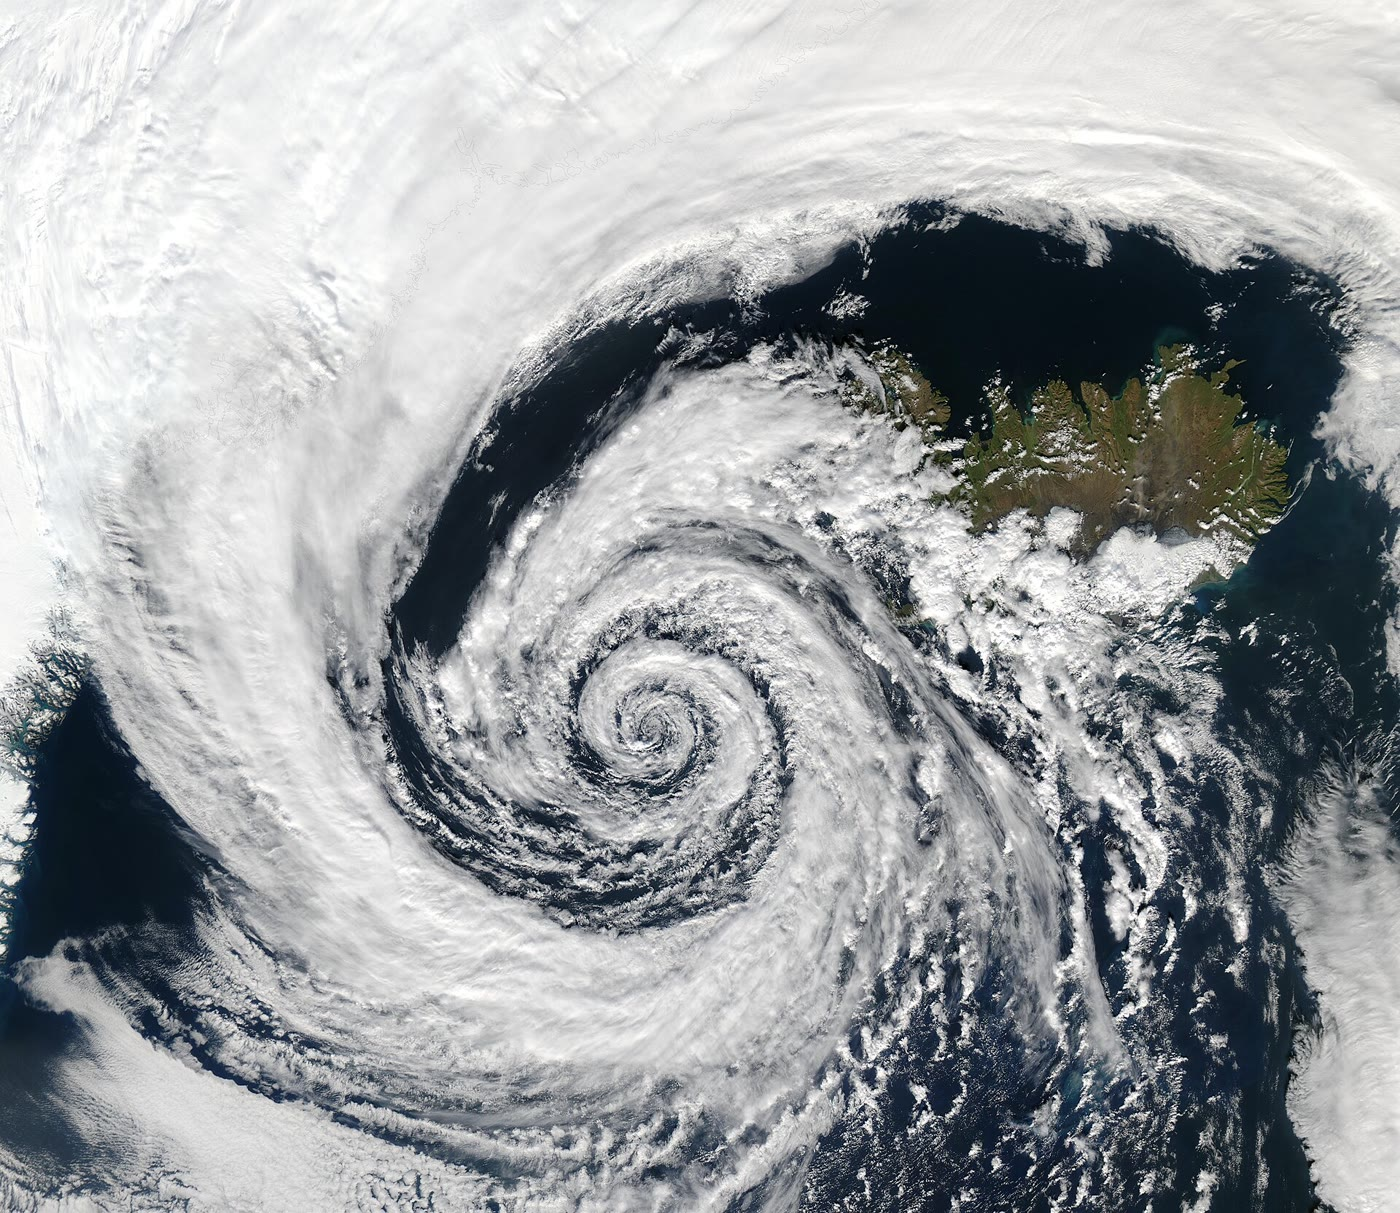
\includegraphics[width=\linewidth]{images/book1/g8-iceland-low.jpg}
\end{minipage}\hfill
\begin{minipage}[c]{0.6\linewidth}\raggedright
{\small Een \omterm{def:g8:fronts-and-weather-maps:depression}{depressie} ten zuidwesten van IJsland (het eiland rechtsboven),
gezien door de satelliet Aqua van de NASA op 4~september 2003. Haar \omterm{def:g4:clouds-rain-snow:cloud}{wolken}
draaien in een spiraal naar het centrum, tegen de klok in, zoals in elke
\omterm{def:g8:fronts-and-weather-maps:depression}{depressie} op het \omterm{def:g3:continents-and-oceans:equator}{noordelijk halfrond}. NASA/GSFC, MODIS Rapid Response Team,
Jacques Descloitres (publiek domein, via Wikimedia Commons).}
\end{minipage}
% ledger: commons:iceland-low, bom:highs-lows
\label{fig:g8:fronts-and-weather-maps:iceland}
\end{omfigure}

\section{Isobaren en weerkaarten}

Om de \omterm{def:g8:fronts-and-weather-maps:depression}{depressies} en \omterm{def:g8:fronts-and-weather-maps:depression}{anticyclonen} te zien, tekenen weervoorspellers \omterm{def:g2:drawing-to-map:map}{kaarten}
van de luchtdruk. Elk station meet zijn druk en herleidt die tot
\omterm{def:g4:world-physical-map:altitude}{zeeniveau}, zodat een station op een \omterm{def:g1:landscapes-around-us:landform}{berg} kan worden vergeleken met een
station aan de \omterm{def:g1:landscapes-around-us:water}{kust}. Dan worden er lijnen getrokken door alle plaatsen
waar de druk gelijk is.
% ledger: bom:isobars

\begin{definition}[Isobaar]\label{def:g8:fronts-and-weather-maps:isobar}
Een \emph{isobaar}\index{isobaar} is een lijn op een \omterm{def:g2:drawing-to-map:map}{kaart} die plaatsen
verbindt waar de druk op \omterm{def:g4:world-physical-map:altitude}{zeeniveau} gelijk is. Isobaren worden gelabeld in
hectopascal en worden vaak om de \qty{4}{hPa} getekend.
\end{definition}
% ledger: bom:isobars (the 4 hPa step is the one of this book's maps)

Rond een \omterm{def:g8:fronts-and-weather-maps:depression}{depressie} vormen de \omterm{def:g8:fronts-and-weather-maps:isobar}{isobaren} gesloten lussen, met de laagste druk
in het centrum, aangeduid met L; rond een \omterm{def:g8:fronts-and-weather-maps:depression}{anticycloon} vormen ze lussen met
de hoogste druk in het centrum, aangeduid met H. Waar de \omterm{def:g8:fronts-and-weather-maps:isobar}{isobaren} dicht
bij elkaar liggen, verandert de druk snel van de ene plaats naar de
volgende en is de wind sterk; waar ze ver uit elkaar liggen, is de wind
zwak.
% ledger: bom:isobars

\begin{omfigure}
\begin{tikzpicture}
\begin{axis}[width=14cm, axis equal image, xmin=0, xmax=2400, ymin=0, ymax=1600,
  hide axis, clip=true, axis background/.style={fill=white}]
  \addplot[isobar] table {figdata/out/grade-8-weather_map-isobars.dat};
  \addplot[warm front] table {figdata/out/grade-8-weather_map-warm.dat};
  \addplot[cold front] table {figdata/out/grade-8-weather_map-cold.dat};
  \addplot[quiver={u=\thisrow{u}, v=\thisrow{v}}, -{Stealth[length=1.5mm]}, omMeth, line width=0.6pt]
    table[x=x, y=y] {figdata/out/grade-8-weather_map-winds.dat};
  \addplot[only marks, mark=none, nodes near coords, point meta=explicit symbolic,
    every node near coord/.style={anchor=center, font=\tiny, fill=white, inner sep=0.6pt}]
    table[x=x, y=y, meta=level] {figdata/out/grade-8-weather_map-labels.dat};
  \node[font=\Large\bfseries, omCold, fill=white, inner sep=1pt] at (axis cs:690,1010) {L};
  \node[font=\scriptsize, anchor=north, fill=white, inner sep=0.5pt] at (axis cs:690,968) {980};
  \node[font=\Large\bfseries, omWarm] at (axis cs:1950,520) {H};
  \node[font=\scriptsize, anchor=north] at (axis cs:1950,485) {1034};
  \addplot[only marks, mark=square*, mark size=2pt, black] table[x=x, y=y] {figdata/out/grade-8-weather_map-town.dat};
  \node[font=\footnotesize\bfseries, anchor=west, fill=white, inner sep=1pt] at (axis cs:870,380) {T};
  \fill[white] (axis cs:1930,1450) rectangle (axis cs:2290,1585);
  \draw[line width=1pt] (axis cs:1950,1480) -- (axis cs:2250,1480);
  \pgfplotsinvokeforeach{1950,2050,2150,2250}{\draw (axis cs:#1,1460) -- (axis cs:#1,1500);}
  \node[font=\scriptsize, anchor=south] at (axis cs:2100,1495) {300 km};
\end{axis}
\end{tikzpicture}

{\small Een weerkaart van een denkbeeldige dag op het \omterm{def:g3:continents-and-oceans:equator}{noordelijk halfrond},
berekend met een model van de luchtdruk. \omterm{def:g8:fronts-and-weather-maps:isobar}{Isobaren} om de \qty{4}{hPa}; de
\omterm{def:g8:fronts-and-weather-maps:depression}{depressie} L (\qty{980}{hPa}) heeft een \omterm{def:g8:fronts-and-weather-maps:front}{warmtefront} (rood) en een \omterm{def:g8:fronts-and-weather-maps:front}{koufront}
(blauw); de \omterm{def:g8:fronts-and-weather-maps:depression}{anticycloon} H (\qty{1034}{hPa}) ligt in het oosten. Groene
pijlen: de wind, langer waar hij sterker is. T: de stad van het probleem.}
% ledger: bom:isobars, bom:highs-lows, mo:fronts (figdata/grade-8/weather_map.py)
\label{fig:g8:fronts-and-weather-maps:map}
\end{omfigure}

\begin{method}[Een weerkaart lezen]
\begin{enumerate}
  \item Zoek de centra: L voor de \omterm{def:g8:fronts-and-weather-maps:depression}{depressies}, H voor de \omterm{def:g8:fronts-and-weather-maps:depression}{anticyclonen},
        met hun druk.
  \item Lees de \omterm{def:g8:fronts-and-weather-maps:isobar}{isobaren}: hun waarden stijgen naar H toe en \omterm{def:g1:landscapes-around-us:landform}{dalen} naar L
        toe. \omterm{def:g8:fronts-and-weather-maps:isobar}{Isobaren} dicht bij elkaar betekenen een sterke wind.
  \item Zoek de richting van de wind: op het \omterm{def:g3:continents-and-oceans:equator}{noordelijk halfrond} waait hij
        bijna langs de \omterm{def:g8:fronts-and-weather-maps:isobar}{isobaren}, met de lage druk aan zijn linkerkant, een
        beetje naar het lagedrukgebied toe gedraaid.
  \item Zoek de \omterm{def:g8:fronts-and-weather-maps:front}{fronten} en de richting waarin ze zich verplaatsen (de kant
        van hun symbolen), en dan de lucht aan elke kant: wat komt er?
\end{enumerate}
\end{method}
% ledger: bom:isobars, bom:highs-lows, mo:fronts

\begin{example}[Het weer in de stad T]
Op de \omterm{def:g2:drawing-to-map:map}{kaart} ligt T ten zuiden van het \omterm{def:g8:fronts-and-weather-maps:front}{warmtefront} en ten oosten van het
\omterm{def:g8:fronts-and-weather-maps:front}{koufront}: in de warme lucht tussen de twee \omterm{def:g8:fronts-and-weather-maps:front}{fronten}. Het \omterm{def:g8:fronts-and-weather-maps:front}{warmtefront} is er
al overheen getrokken. De \omterm{def:g8:fronts-and-weather-maps:isobar}{isobaren} lopen daar van het zuidwesten naar het
noordoosten, met het lagedrukgebied in het noordwesten: de wind waait uit
het zuidwesten, warm en vochtig. Het \omterm{def:g8:fronts-and-weather-maps:front}{koufront} komt uit het westen. Zijn
driehoekjes wijzen naar het oosten, naar de stad: binnen enkele uren komt
er een korte periode met hevige buien en windstoten, daarna draait de wind
naar het westen of noordwesten, wordt het koeler en klaart de lucht op.
\end{example}
% ledger: ucar:cold-front (figdata/grade-8/weather_map.py: wind at T from 227 degrees)

Een barometer geeft zijn eigen waarschuwing, ook zonder \omterm{def:g2:drawing-to-map:map}{kaart}. Stel dat de
hele \omterm{def:g2:drawing-to-map:map}{kaart} hierboven zonder te veranderen met \qty{40}{km} per uur naar het
oosten schoof, en dat er een registrerende barometer stond in een station
S, ten oosten van de \omterm{def:g8:fronts-and-weather-maps:front}{fronten}. In tweeënhalve dag zou hij de registratie
hieronder tekenen.

\begin{omfigure}
\begin{tikzpicture}
\begin{axis}[width=0.86\linewidth, height=5.4cm, xmin=0, xmax=60, ymin=980, ymax=1040,
  xtick={0,12,...,60}, ytick={980,990,...,1040},
  xlabel={uren sinds het begin van de registratie}, ylabel={druk (hPa)},
  axis x line=bottom, axis y line=left, axis line style={-},
  grid=major, grid style={black!10},
  tick label style={font=\scriptsize}, label style={font=\small}, clip=false]
  \draw[omWarm!80!black, dashed] (axis cs:26.28,980) -- (axis cs:26.28,1040);
  \draw[omCold!80!black, dashed] (axis cs:38.49,980) -- (axis cs:38.49,1040);
  \node[font=\scriptsize, omWarm!80!black, anchor=south, fill=white, inner sep=1pt] at (axis cs:26.28,1032) {warmtefront};
  \node[font=\scriptsize, omCold!80!black, anchor=south, fill=white, inner sep=1pt] at (axis cs:38.49,1032) {koufront};
  \addplot[black!80, line width=1pt] table[x=hour, y=p_hPa] {figdata/out/grade-8-barogram-trace.dat};
  \node[font=\scriptsize, anchor=north west, align=left] at (axis cs:2,1028) {anticycloon:\\rustig};
  \node[font=\scriptsize, anchor=west] at (axis cs:39.5,986) {laagste};
\end{axis}
\end{tikzpicture}

{\small De registratie van een barometer in het station S terwijl de \omterm{def:g2:drawing-to-map:map}{kaart}
hierboven met \qty{40}{km} per uur naar het oosten schuift (een verzonnen
situatie, berekend met het drukveld van de \omterm{def:g2:drawing-to-map:map}{kaart}). Stippellijnen: het
\omterm{def:g8:fronts-and-weather-maps:front}{warmtefront} en het \omterm{def:g8:fronts-and-weather-maps:front}{koufront} die over het station trekken.}
% ledger: (invented region: weather situation of figdata/grade-8/weather_map.py, record from figdata/grade-8/barogram.py)
\end{omfigure}

\begin{example}[Een barometerregistratie lezen]\label{ex:g8:fronts-and-weather-maps:barogram}
De eerste 8 uur stijgt de druk tot ongeveer \qty{1031}{hPa}: de \omterm{def:g8:fronts-and-weather-maps:depression}{anticycloon}
trekt over S, met rustig \omterm{def:g1:watching-the-weather:weather}{weer}. Dan daalt hij 30 uur lang, met ongeveer
\qty{45}{hPa}: de \omterm{def:g8:fronts-and-weather-maps:depression}{depressie} komt eraan. Hij daalt het snelst een paar uur
voordat het \omterm{def:g8:fronts-and-weather-maps:front}{warmtefront} passeert, langzamer in de warme lucht erachter, en
bereikt zijn laagste waarde, ongeveer \qty{986}{hPa}, precies als het
\omterm{def:g8:fronts-and-weather-maps:front}{koufront} passeert. Dan stijgt hij: de \omterm{def:g8:fronts-and-weather-maps:depression}{depressie} trekt weg, en de koelere,
helderdere lucht achter het \omterm{def:g8:fronts-and-weather-maps:front}{koufront} komt eraan.
% ledger: (invented region: figdata/grade-8/barogram.py), bom:highs-lows
\end{example}

\section{Hoe een weersverwachting wordt gemaakt}

\begin{definition}[Weersverwachting]\label{def:g8:fronts-and-weather-maps:forecast}
Een \emph{weersverwachting}\index{weersverwachting} is een uitspraak over
het \omterm{def:g1:watching-the-weather:weather}{weer} dat op een plaats in de komende uren of dagen wordt verwacht,
opgesteld uit waarnemingen van de atmosfeer en met de wetten van de
natuurkunde.
\end{definition}
% ledger: mo:how-forecasts

Een \omterm{def:g8:fronts-and-weather-maps:forecast}{weersverwachting} wordt in drie stappen gemaakt. Eerst doen
weerdiensten over de hele wereld elke dag miljoenen waarnemingen:
temperatuur, \omterm{def:g4:clouds-rain-snow:precipitation}{neerslag}, luchtdruk, wind en vochtigheid, gemeten op
grondstations, op \omterm{def:g2:water-on-earth:ocean}{zee}, met weerballonnen, met radar en vanuit satellieten.
Dan worden deze waarnemingen ingevoerd in computermodellen: heel krachtige
computers berekenen stap voor stap hoe de atmosfeer vanuit haar huidige
toestand zal veranderen. Ten slotte lezen weervoorspellers de resultaten,
vergelijken ze die met wat ze van hun regio weten, en schrijven ze de
\omterm{def:g8:fronts-and-weather-maps:forecast}{weersverwachting}.
% ledger: mo:how-forecasts

\begin{history}[De eerste openbare weersverwachting]
In 1854 werd een marineofficier, Robert FitzRoy, aan het hoofd gezet van
een nieuw weerbureau in Londen. Elke ochtend om 9~uur maten stations langs
de \omterm{def:g1:landscapes-around-us:water}{kusten} het \omterm{def:g1:watching-the-weather:weather}{weer} en stuurden ze hun waarnemingen naar Londen met de
telegraaf, de nieuwste uitvinding van die tijd. In 1859 bracht een
verschrikkelijke \omterm{def:g5:natural-hazards:storm}{storm}, de \omterm{def:g5:natural-hazards:storm}{storm} van de \emph{Royal Charter}, veel schepen
tot zinken; FitzRoy richtte toen een dienst van stormwaarschuwingen voor
zeelieden op, die in februari 1861 begon. Op 1~augustus 1861 ging hij
verder en publiceerde hij de eerste openbare \omterm{def:g8:fronts-and-weather-maps:forecast}{weersverwachting} in een krant,
\emph{The Times}. Zijn verwachtingen keken een of twee dagen vooruit en
waren heel algemeen; ze waren het begin van de \omterm{def:g8:fronts-and-weather-maps:forecast}{weersverwachtingen} die we
nu lezen.
\end{history}
% ledger: mo:fitzroy

\omterm{def:g8:fronts-and-weather-maps:forecast}{Weersverwachtingen} zijn veel beter geworden. In de afgelopen decennia
hebben weervoorspellers er ongeveer elke tien jaar een dag goede
verwachting bij gewonnen: een verwachting voor vier dagen vooruit is nu
even goed als een verwachting voor één dag vooruit dertig jaar geleden.
Maar hoe verder een verwachting vooruitkijkt, hoe minder zeker ze is,
omdat kleine fouten in de beginwaarnemingen groeien naarmate de computer
verder in de tijd rekent.
% ledger: bauer:day-per-decade, mo:accuracy

\begin{inthefield}[Een front zien aankomen]
Kijk op een dag waarop de \omterm{def:g8:fronts-and-weather-maps:forecast}{weersverwachting} een \omterm{def:g8:fronts-and-weather-maps:front}{front} aankondigt om de paar
uur naar de lucht en noteer de tijd, de \omterm{def:g4:clouds-rain-snow:cloud}{wolken}, de wind en de temperatuur.
Komen er voor een \omterm{def:g8:fronts-and-weather-maps:front}{warmtefront} eerst hoge strepen \omterm{def:g4:clouds-rain-snow:cloud-families}{cirrus}? Daalt de
temperatuur en verandert de wind als er een \omterm{def:g8:fronts-and-weather-maps:front}{koufront} passeert? Vergelijk
je aantekeningen met de weerkaart van die dag.
\end{inthefield}

\section{Oefeningen}

\begin{exercise}[$\star$]\label{exo:g8:fronts-and-weather-maps:1}
Geef de betekenis van elk paar letters en zeg of de \omterm{def:g8:fronts-and-weather-maps:air-mass}{luchtmassa} warm of
koud, vochtig of droog is: (a) mT; (b) cP; (c) cT; (d) mP.
\end{exercise}

\begin{exercise}[$\star$]\label{exo:g8:fronts-and-weather-maps:2}
Koppel elk teken van een weerkaart aan zijn betekenis: een blauwe lijn met
driehoekjes; een rode lijn met halve cirkels; een lijn die plaatsen met
dezelfde druk verbindt; de letter H; de letter L.
\end{exercise}

\begin{exercise}[$\star$]\label{exo:g8:fronts-and-weather-maps:3}
Waar of niet waar? Verbeter de onware zinnen. (a) \omterm{def:g8:fronts-and-weather-maps:depression}{Anticyclonen} brengen
meestal rustig \omterm{def:g1:watching-the-weather:weather}{weer}. (b) De \omterm{def:g4:clouds-rain-snow:cloud}{wolken} van een \omterm{def:g8:fronts-and-weather-maps:front}{warmtefront} komen na het \omterm{def:g8:fronts-and-weather-maps:front}{front}.
(c) \omterm{def:g8:fronts-and-weather-maps:isobar}{Isobaren} dicht bij elkaar betekenen een zwakke wind. (d) Koude lucht
is dichter dan warme lucht.
\end{exercise}

\begin{exercise}[$\star$]\label{exo:g8:fronts-and-weather-maps:4}
Op de weerkaart van dit hoofdstuk: (a) wat is de druk in het centrum van de
\omterm{def:g8:fronts-and-weather-maps:depression}{depressie}? (b) En van de \omterm{def:g8:fronts-and-weather-maps:depression}{anticycloon}? (c) Hoeveel hectopascal ligt er
tussen twee naburige \omterm{def:g8:fronts-and-weather-maps:isobar}{isobaren}? (d) Hoeveel hectopascal verschilt de druk
tussen de twee centra?
\end{exercise}

\begin{exercise}[$\star\star$]\label{exo:g8:fronts-and-weather-maps:5}
Zet deze gebeurtenissen in de volgorde waarin ze plaatsvinden als een
\omterm{def:g8:fronts-and-weather-maps:front}{warmtefront} nadert en voorbijtrekt: gestage \omterm{def:g4:clouds-rain-snow:precipitation}{regen}; dunne strepen \omterm{def:g4:clouds-rain-snow:cloud-families}{cirrus};
een grijze sluier van altostratus; warmere, vochtigere lucht; de \omterm{def:g4:clouds-rain-snow:cloud}{wolken}
komen lager en worden dikker.
\end{exercise}

\begin{exercise}[$\star\star$]\label{exo:g8:fronts-and-weather-maps:6}
Leg uit waarom de \omterm{def:g4:clouds-rain-snow:cloud}{wolken} van een \omterm{def:g8:fronts-and-weather-maps:front}{koufront} hoog oprijzen, terwijl die van
een \omterm{def:g8:fronts-and-weather-maps:front}{warmtefront} in lagen zijn uitgespreid. Gebruik de woorden \emph{wig},
\emph{steil}, \emph{flauwe helling}.
\end{exercise}

\begin{exercise}[$\star\star$]\label{exo:g8:fronts-and-weather-maps:7}
Op de weerkaart: (a) waar is de wind het sterkst, bij L of bij H? Hoe zie
je dat? (b) Uit welke richting waait de wind ten noorden van L? (c) En ten
zuiden van H? (d) Draait de wind met de klok mee of tegen de klok in om L?
\end{exercise}

\begin{exercise}[$\star\star$]\label{exo:g8:fronts-and-weather-maps:8}
Een barometer in een stad wijst om 6.00~uur \qty{1016}{hPa} aan, om
12.00~uur \qty{1009}{hPa} en om 18.00~uur \qty{1003}{hPa}. (a) Hoeveel
daalt de druk in 12 uur? (b) Wat komt er naar de stad toe, een \omterm{def:g8:fronts-and-weather-maps:depression}{depressie} of
een \omterm{def:g8:fronts-and-weather-maps:depression}{anticycloon}? (c) Welk \omterm{def:g1:watching-the-weather:weather}{weer} kan de stad verwachten?
\end{exercise}

\begin{exercise}[$\star\star$]\label{exo:g8:fronts-and-weather-maps:9}
Lucht die een week boven de Sahara heeft gehangen, trekt naar het noorden
over de Middellandse \omterm{def:g2:water-on-earth:ocean}{Zee}. (a) Geef deze \omterm{def:g8:fronts-and-weather-maps:air-mass}{luchtmassa} haar naam van twee
letters. (b) Is ze heet of koud, vochtig of droog, als ze vertrekt?
(c) Wat zou er aan haar karakter kunnen veranderen terwijl ze de \omterm{def:g2:water-on-earth:ocean}{zee}
oversteekt?
\end{exercise}

\begin{exercise}[$\star\star$]\label{exo:g8:fronts-and-weather-maps:10}
Een verwachting voor vier dagen vooruit is nu even goed als een
verwachting voor één dag vooruit dertig jaar geleden. (a) Hoeveel dagen
goede verwachting zijn er in dertig jaar gewonnen? (b) Hoeveel is dat per
tien jaar? (c) Als dezelfde vooruitgang doorging, over hoeveel jaar zou een
verwachting voor vijf dagen dan even goed zijn als de verwachting voor één
dag van nu?
\end{exercise}

\begin{exercise}[$\star\star\star$]\label{exo:g8:fronts-and-weather-maps:11}
Gebruik op de weerkaart de schaalbalk. (a) Ongeveer hoeveel kilometer ligt
er tussen het centrum L en het centrum H? (b) Bij L liggen twee naburige
\omterm{def:g8:fronts-and-weather-maps:isobar}{isobaren} ongeveer \qty{80}{km} uit elkaar. Met hoeveel hectopascal
verandert de druk daar over \qty{100}{km}? (c) Bij H liggen twee naburige
\omterm{def:g8:fronts-and-weather-maps:isobar}{isobaren} ongeveer \qty{140}{km} uit elkaar. Zelfde vraag. (d) Waar is de
wind sterker? Komen de pijlen op de \omterm{def:g2:drawing-to-map:map}{kaart} daarmee overeen?
\end{exercise}

\begin{exercise}[$\star\star\star$]\label{exo:g8:fronts-and-weather-maps:12}
Een \omterm{def:g8:fronts-and-weather-maps:front}{koufront} ligt \qty{300}{km} ten westen van een stad en verplaatst zich
met \qty{50}{km} per uur naar het oosten; een \omterm{def:g8:fronts-and-weather-maps:front}{warmtefront} ligt
\qty{200}{km} ten westen van een andere stad en verplaatst zich met de
helft van die snelheid. (a) Welk \omterm{def:g8:fronts-and-weather-maps:front}{front} bereikt zijn stad het eerst, en
hoeveel uur eerder? (b) Beschrijf het \omterm{def:g1:watching-the-weather:weather}{weer} dat elke stad zal zien als haar
\omterm{def:g8:fronts-and-weather-maps:front}{front} passeert. (c) Welke stad zal warmer zijn als haar \omterm{def:g8:fronts-and-weather-maps:front}{front} voorbij is?
\end{exercise}

\section{Probleem: Gaat de wedstrijd door de regen niet door?}

\begin{problem}[{Weekendprobleem --- een voetbalwedstrijd staat om
15.00~uur gepland in de stad T van de weerkaart; het koufront komt eraan:
zijn snelheid wordt op twee kaarten gemeten en het uur waarop het de stad
bereikt wordt voorspeld}]
\label{pb:g8:fronts-and-weather-maps:1}
% ledger: ucar:cold-front (figdata/grade-8/weather_map.py; the front's speed and the length of the showers are exercise data)
Om 9.00~uur kijkt een jonge weervoorspeller naar de weerkaart van dit
hoofdstuk en daarna naar de \omterm{def:g2:drawing-to-map:map}{kaart} hieronder: die toont het \omterm{def:g8:fronts-and-weather-maps:front}{koufront} bij de
stad om 6.00~uur en om 9.00~uur, op een rooster van hokjes van
\qty{20}{km}.

\begin{center}
\begin{tikzpicture}
\begin{axis}[width=11cm, axis equal image, xmin=0, xmax=600, ymin=0, ymax=400,
  xtick={0,100,...,600}, ytick={0,100,...,400}, minor tick num=4,
  grid=both, minor grid style={black!10}, major grid style={black!25},
  tick label style={font=\scriptsize}, xlabel={afstand naar het oosten (km)}, ylabel={afstand naar het noorden (km)},
  label style={font=\small}]
  \addplot[cold front, densely dashed, opacity=0.55] table[x expr=\thisrow{x}-363.2, y expr=\thisrow{y}-180] {figdata/out/grade-8-weather_map-seq-06.dat};
  \addplot[cold front] table[x expr=\thisrow{x}-363.2, y expr=\thisrow{y}-180] {figdata/out/grade-8-weather_map-seq-09.dat};
  \addplot[only marks, mark=square*, mark size=2.2pt, black] table[x expr=\thisrow{x}-363.2, y expr=\thisrow{y}-180] {figdata/out/grade-8-weather_map-town.dat};
  \node[font=\footnotesize\bfseries, anchor=south west, fill=white, inner sep=1pt] at (axis cs:485,205) {T};
  \node[font=\scriptsize, fill=white, inner sep=1pt] at (axis cs:140,360) {06.00};
  \node[font=\scriptsize, fill=white, inner sep=1pt] at (axis cs:262,360) {09.00};
\end{axis}
\end{tikzpicture}
\end{center}

\noindent\textbf{Deel I --- De kaart lezen.}\par\nopagebreak
\begin{enumerate}[beginpenalty=10000]
  \item Ligt de stad op de weerkaart van het hoofdstuk in de warme lucht of
        in de koude lucht? Welk \omterm{def:g8:fronts-and-weather-maps:front}{front} is er al overheen getrokken?
  \item Uit welke richting waait de wind in de stad?
  \item In welke richting verplaatst het \omterm{def:g8:fronts-and-weather-maps:front}{koufront} zich? Hoe zie je dat aan
        zijn symbolen?
  \item Welk \omterm{def:g1:watching-the-weather:weather}{weer} zal het \omterm{def:g8:fronts-and-weather-maps:front}{koufront} brengen als het passeert?
\end{enumerate}

\noindent\textbf{Deel II --- De snelheid van het front.}\par\nopagebreak
\begin{enumerate}[resume, beginpenalty=10000]
  \item Hoe ver naar het oosten ligt het \omterm{def:g8:fronts-and-weather-maps:front}{front} op de \omterm{def:g2:drawing-to-map:map}{kaart} hierboven, op
        de hoogte van de stad, om 6.00~uur? En om 9.00~uur?
  \item Hoeveel kilometer heeft het \omterm{def:g8:fronts-and-weather-maps:front}{front} zich in deze drie uur verplaatst?
  \item Wat is zijn snelheid, in kilometer per uur?
  \item Hoeveel kilometer ligt er om 9.00~uur tussen het \omterm{def:g8:fronts-and-weather-maps:front}{front} en de stad?
\end{enumerate}

\noindent\textbf{Deel III --- De verwachting.}\par\nopagebreak
\begin{enumerate}[resume, beginpenalty=10000]
  \item Als het \omterm{def:g8:fronts-and-weather-maps:front}{front} dezelfde snelheid houdt, hoeveel uur heeft het dan
        nodig om de stad te bereiken?
  \item Hoe laat bereikt het de stad?
  \item Stel dat de hevige buien ongeveer een uur aanhouden nadat het \omterm{def:g8:fronts-and-weather-maps:front}{front}
        is gepasseerd. Regent het dan om 15.00~uur nog?
  \item Het \omterm{def:g8:fronts-and-weather-maps:front}{front} zou kunnen vertragen tot \qty{30}{km} per uur. Wanneer
        zou het de stad dan bereiken? Schrijf de verwachting voor de
        wedstrijd in een of twee zinnen, met beide mogelijke tijdstippen.
\end{enumerate}
\end{problem}
